\documentclass[12pt, a4paper]{article}

\usepackage[slovene, english]{babel}
\usepackage[utf8]{inputenc}
\usepackage{amsmath, amsfonts}
\usepackage{url}
\usepackage{graphicx}
%\usepackage{tikz}
\usepackage{textpos}
\usepackage{wrapfig}
\usepackage{amsthm}
%\usepackage{enumitem}

\newtheorem{izrek}{Izrek}
\newtheorem{zgled}{Zgled}
\newtheorem{trditev}{Trditev}
\newtheorem{lema}{Lema}
\newtheorem{definicija}{Definicija}
\newtheorem{pos}{Posledica}

\newcommand{\R}{\mathbb R}
\newcommand{\N}{\mathbb N}
\newcommand{\Z}{\mathbb Z}
\newcommand{\C}{\mathbb C}
\newcommand{\Q}{\mathbb Q}

\renewcommand{\mod}{\operatorname{mod}}

\title{Zadnji Fermatov izrek za $n=4$}
\author{Ajda Frankovič, Jernerj Grlj, Gregor Kikelj \\ Mentor: Rok Havlas}
%\date%{
\includegraphics[width = 6cm]{logo_MaRS2017.png}}

\selectlanguage{slovene}

\begin{document}


\begin{abstract}
kk
\end{abstract}

\section{Uvod}




\newpage
\section{Funkcije dveh spemenljivk}


\begin{definicija}
\textbf{Funkcija dveh neodvisnih spremenljivk} je predpis, ki vsakemu paru $(x,y)$ iz podmnožice ravnine predpiše natančno določeno realno število.
Je preslikava $R^2 \rightarrow R$.
$$f:(x,y) \Rightarrow z=f(x,y)$$

\end{definicija}

Realno število, ki je prirejeno spremenljivkam v trorazsežnem prostoru pomeni višino nad točko. Upodabljamo lahko le funkcije z do tremimi spremenljivkami, za sistem štirih ali večih spemenljivk pa je upodabljanje nemogoče. Za razliko od funkcij z eno spremenljivko upodabljamo funkcije dveh spremenljivk s ploskvijo, ki ima enačbo $u-f(x,y)=0$. Spoznali smo nekaj preprostih funkcij, ogledali pa smo si tudi primere zahtevnejših funkcij dveh spremenljivk.

\begin{zgled}
Funkcija $f(x,y)=x^2+y^2$ Graf funkcije je dvorazsežni objekt v trorazsežnem prostoru.
\end{zgled}

\begin{figure}[h!]
\centering
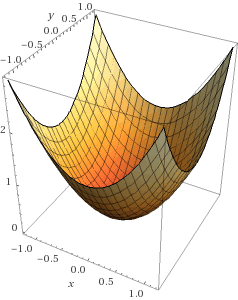
\includegraphics{slika_funkcije.PNG}
\caption{Graf funkcije f(x,y)}
\end{figure}

\newpage
\begin{zgled}
Primer zahtevnejše funkcije $g(x,y)=x^2 sin(x)y^3$ 
\end{zgled}

\begin{figure}[h!]
\centering
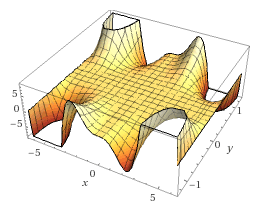
\includegraphics{funkcija_2.PNG}
\caption{Graf funkcije g(x,y)}
\end{figure}


\section{Volumen krogle}

Izračunali smo tudi volumen krogle z različnimi metodami: 

\begin{zgled} 
Izračun prostornine vrtenine, ki nastane z vrtenjem funkcije $f(x)=\sqrt{(1-x^2)}$ .

$$V=\pi \int_{a}^b{f(x)}^2dx$$
$$V=\pi \int_{-1}^1{{\sqrt{(1-x^2)}}}^2dx=\pi(x-\frac{x^3}{3})\mid_{-1}^1= \pi (1-\frac{1}{3})-\pi (-1+\frac{1}{3})$$
$$V=\frac{4}{3}\pi$$
\end{zgled}

\newpage
\section{Računanje determinante reda 2 in 3}

Poglejmo si kako se računa determinanta reda 2 in 3. Tukaj so eksplicitne formule za njihov izračun.

\[
\begin{vmatrix}
    a& b  \\
   c &d \\
\end{vmatrix}
=ad-bc
\]

\[
\begin{vmatrix}
 a&b&c\\
 d&e&f\\
 g&h&i\\
\end{vmatrix}
=a\begin{vmatrix}
e&f\\
h&i\\
\end{vmatrix}-b\begin{vmatrix}
d&f\\
g&i\\
\end{vmatrix}+c\begin{vmatrix}
d&e\\
g&h\\
\end{vmatrix}
\]

\section{Zamenjava spremenljivke v integralu}
Najprej se bomo seznanili s primerom zamenjave ene spremenljivke potem pa bomo spoznali še zamenjavo dveh in treh spremenljivk v integralu.
\\
Naj bo $f$ zvezna na $[a,b]$ in $\phi$ zvezno odvedljiva funkcija, ki interval $[\alpha,\beta]$ preslika bijektivno na interval $[a,b]$ tako, da je  $\phi(\alpha)=a$ in $\phi(\beta)=b$. Tedaj je

$$\int_{a}^bf(x)\mathrm{d} x=\int_{\alpha}^{\beta}f(\phi(t))\phi'(t)\mathrm{d} t$$

Na podoben način lahko zamenjamo več spremenljivk. Naj bo $U \subset \mathbb{R}^n$ odprta množica z volumnom $\neq 0$ in $g:U \rightarrow \mathbb{R}^n$ dovolj lepa preslikava.
\begin{izrek}
 Naj bo $\big | \det Dg(t) \big |\neq 0$ za vse $t \in U$ in omejena na $U$. Predpostavimo, da ima $g(U)$ volumen. Za vsako integrabilno funkcijo $f:g(U) \rightarrow \mathbb{R}$ velja:

$$\int_{g(U)}^{}f(x) \mathrm{d} V=\int_{U}^{}f(g(t)) \big |\det Dg(t) \big | \mathrm{d} V$$
\end{izrek}

\end{document}